\section{从RGB到HSI的转换}

RGB模型是根据单位立方体定义的.然而, HSI模型的颜色分量(色相和饱和度)是根据图~\ref{fig:-1a} 所示的颜色三角形来定义的.在图~\ref{fig:-1a} 中,注意到色点$P$的色调$H$是所示矢量相对于红原色轴的角度.因此,当$H=0^{\circ}$时,颜色为红色.当$H$为$60^{\circ}$时,颜色为黄色,以此类推.色点$P$的饱和度$S$是颜色未被白色稀释的程度,与$P$到三角形中心的距离成正比. $P$距离三角形中心越远,它的颜色越饱和.

在HSI模型中,强度是根据一条垂直于三角形并通过其中心的线来测量的.沿着三角形下面这条线的强度趋于从暗到黑.相反,在三角形以上的强度则从亮到白.



\begin{figure}[htbp]
  \centering
  \subfigure[\label{fig:-1a}]{
    \begin{tikzpicture}[scale=3,semithick]
      \pgfmathsetmacro{\r}{1}
      \coordinate (W) at (0,0);

      \draw (W) -- (0,\r)  coordinate (PB)node[above] {Blue};
      \draw (W) -- (210:\r) coordinate (PR) node[below left] {Red};
      \draw (W) -- (-30:\r) coordinate (PG) node[below right] {Green};
      \draw (PR)--(PG)--(PB)--cycle;
      \coordinate (QR) at (30:0.5) ;\node[above right] at (QR) {Cyan};
      \coordinate (QG) at (150:0.5);\node[above left] at(QG) {Magenta};
      \coordinate (QB) at (-90:0.5);\node[below] at(QB) {Yellow};

      \fill (W) -- +(-120:0.4) coordinate (P) circle [radius=0.4pt,fill=black] node[below] {$P$};
      \draw[arrows={-Stealth[inset=0pt, angle=25:6pt]}] (W) -- (P);
      \draw[arrows={-Stealth[inset=0pt, angle=25:6pt]}] (-150:0.2) arc[start angle=-150, end angle=-120, radius=0.2];
      \node at (-135:0.3) {$H$};
      \draw[white] (0,-1)--(0,-1.5);
    \end{tikzpicture}
  }\quad
  \subfigure[\label{fig:-1b}]{
    \begin{tikzpicture}[scale=3,semithick]
      \pgfmathsetmacro{\r}{1}
      \coordinate (O1) at (0,0);
      \coordinate (K) at (0,-2);
      \draw (K) node[below] {Black};

      \draw (O1) + (0,\r)  coordinate (W) node[above] {White};
      \draw (O1) + (210:\r) coordinate (R) node[below left] {Red};
      \draw (O1) + (-30:\r) coordinate (G) node[below right] {Green};
      \draw (R)--(W)--(G);
      \draw (R)--(K)--(G);

      \coordinate (U1) at (0,-0.3125) ;
      \coordinate (C) at (0,-0.5) ;
      \coordinate (B) at (0,-0.125) ;
      \draw (B) node[above right] {Blue};
      \draw[very thick] (R)--(G) (G) -- (B) (B)--(R);
      \draw (U1) -- (R) (U1) -- (G);
      \coordinate (U2) at (0,0.22) ;
      \coordinate (U3) at (0,0.1) ;
      \coordinate (G') at (0.5196,0.1) ;
      \coordinate (R') at (-0.5196,0.1) ;
      \coordinate (B') at (0,0.275) ;
      \draw[very thick] (R')--(G') (G')--(B') (B')--(R');
      \draw (W)--(U2) (U3)--(U1);
      \draw[densely dashed] (U2)-- (U3) (U1)--(C);
      \begin{scope}[yshift=-1.2cm]
        \coordinate (G') at (0.5196,0.1) ;
        \coordinate (R') at (-0.5196,0.1) ;
        \coordinate (B') at (0,0.275) ;
        \draw[very thick] (R')--(G') (G')--(B') (B')--(R');
      \end{scope}
      \draw (C)--+(0,-0.48) coordinate (D1);
      \draw[densely dashed] (D1) -- +(0,-0.12) coordinate (D2);
      \draw (D2) -- (K);

      \fill (U1) -- +(-120:0.15) coordinate (P) circle [radius=0.4pt,fill=black];
      \draw[arrows={-Stealth[inset=0pt, angle=25:4pt]}] (U1) -- (P);
      \draw[arrows={-Stealth[inset=0pt, angle=25:4pt]}] (U1)+(-170:0.1) arc[start angle=-150, end angle=-125, radius=0.2];
      \draw (U1)+(-145:0.2) node {$H$};

      \draw (W)--+(1.5,0) coordinate (W1) (K) -- +(1.5,0) coordinate (K1) ;
      \draw (W1)+(-0.2,-1) node (I) {Intensity};
      \draw[arrows={-Stealth[inset=0pt, angle=25:6pt]}] (I.north)-- ($(W1)+(-0.2,0)$);
      \draw[arrows={-Stealth[inset=0pt, angle=25:6pt]}] (I.south)-- ($(K1)+(-0.2,0)$);
    \end{tikzpicture}
  }
  \caption{(a)三角形HSI颜色模型; (b)HSI颜色锥体.}
  \label{fig:-1}
\end{figure}

在三维色彩空间中结合色相、饱和度和强度可以得到图~\ref{fig:-1b} 所示的三面金字塔状结构.这个结构表面的任何一点都代表了一种纯饱和的颜色.该颜色的色调取决于它相对于红原色轴的角度,其强度取决于它与黑色点的垂直距离(也就是说,与黑色的距离越大,该颜色的强度越大).类似的结论也适用于结构内部的点,唯一的区别是颜色在接近垂直轴时变得不那么饱和.

HSI模型中的颜色是根据归一化后的红色、绿色和蓝色值定义的,以RGB原色给出\footnote{参考Gonzalez and Woods, Digital Image Processing, 1st ed. Addison-Wesley, 1992.}
\begin{equation}\label{equ:1}
  r=\frac{R}{R+G+B}\,,
\end{equation}
\begin{equation}\label{equ:2}
  g=\frac{G}{R+G+B}\,,
\end{equation}
\begin{equation}\label{equ:3}
  b=\frac{B}{R+G+B}\,,
\end{equation}
故$r,g,b\in [0,1]$,且
\begin{equation}\label{equ:rgbn}
  r+g+b=1\,.
\end{equation}
注意, 虽然$R,G$和$B$能同时达到最大值,但归一化值仍满足式\eqref{equ:rgbn}.事实上,这个方程的平面包含了HSI三角形.

对于任意的$R,G$和$B$分量,每一个在范围$[0,1]$内, HSI的强度分量定义为
\begin{equation}\label{equ:I}
  I=\frac{1}{3}(R+G+B)\,,
\end{equation}
其值在$[0,1]$范围内.

下一步是获得$H$和$S$分量,为了从图~\ref{fig:0} 的几何约束中得到$H$,我们作如下条件说明:

\begin{figure}[t]
  \centering
  \subfigure[\label{fig:0a}]{
    \begin{tikzpicture}[scale=3,semithick]
    \pgfmathsetmacro{\r}{1}
    \coordinate (W) at (0,0); \draw (W)+(60:0.15) node {$W$};

    \draw (W) -- (0,\r)  coordinate (PB)node[above] {$P_B$};
    \draw (W) -- (210:\r) coordinate (PR) node[below left] {$P_R$};
    \draw (W) -- (-30:\r) coordinate (PG) node[below right] {$P_G$};
    \draw (PR)--(PG)--(PB)--cycle;
    \coordinate (QR) at (30:0.5) ;\node[above right] at (QR) {$Q_R$};
    \coordinate (QG) at (150:0.5);\node[above left] at(QG) {$Q_G$};
    \coordinate (QB) at (-90:0.5);\node[below] at(QB) {$Q_B$};
    \draw (W)--(QR) (W)--(QG) (W)--(QB);

    \fill (W) -- +(-120:0.577) coordinate (P') circle [radius=0.4pt,fill=black] node[below] {$P'$};
    \fill (W) -- +(-120:0.4) coordinate (P) circle [radius=0.4pt,fill=black] node[below] {$P$};
    \draw[arrows={-Stealth[inset=0pt, angle=25:6pt]}] (W) -- (P);
    \draw (P)--(P');
    \draw[arrows={-Stealth[inset=0pt, angle=25:6pt]}] (-150:0.2) arc[start angle=-150, end angle=-120, radius=0.2];
    \node at (-135:0.3) {$H$};
      \end{tikzpicture}
  }

  \subfigure[\label{fig:0b}]{
      \begin{tikzpicture}[scale=3,semithick]
        % 坐标原点
        \coordinate (O) at (0,0);
        % \node[above left] at (O) {$O$};
    
        % 坐标系
        \draw [dashed] (O) -- (0,1) coordinate(PB) node[above left]  {$P_B$} node[above right] {$(0,0,1)$};
        \draw [arrows={-Stealth}] (PB) -- (0,1.3) node[anchor=south]  {$b$};
        \draw [dashed] (O) -- (1,0) coordinate(PG) node[below right]  {$P_G$} node[above right] {$(0,1,0)$};
        \draw [arrows={-Stealth}] (PG) -- (1.3,0) node[below] {$g$};
        \draw [dashed] (O) -- (-0.6,-0.9) coordinate(PR) node[above left]  {$P_R$} node[below right] {$(1,0,0)$};
        \draw [arrows={-Stealth}] (PR) -- (-0.75,-1.125) node[below] {$r$};

        \draw (PB)--(PR)--(PG)--cycle;
        % \fill (0.5,0.5) coordinate (QR) circle [radius=0.4pt,fill=black] node [above right] {$Q_R$};
        % \draw (PR) -- (QR) ;
        \fill (0.2,0.118) coordinate (W) circle [radius=0.4pt,fill=black] node[above] {$W$};
        \fill (W) -- + (-100:0.64) coordinate (P') circle [radius=0.4pt,fill=black] node[below] {$P'$} ;
        \fill (W) -- + (-100:0.32) coordinate (P) circle [radius=0.4pt,fill=black] node[left] {$P$} ;
        \draw (W) -- (P');
        \fill (W) -- +(0,-0.4) coordinate (T) circle [radius=0.4pt,fill=black] node[below] {$T$};
        \draw[densely dashed] (W) -- (T);
        \draw [densely dashed] (T) -- +(-0.4,0) node[above left,inner sep=0pt] {$1\,/\,3$};
        \draw [densely dashed] (T) -- (0.4,0); \draw (0.45,0) node[above] {$1\,/\,3$};
        \fill (P) -- +(65:0.13) coordinate (Q) circle [radius=0.4pt,fill=black] node[right,inner sep=1pt] {$Q$} ;
        \draw[densely dashed] (P) -- (Q) ;
      \end{tikzpicture}
  }
  \qquad
  \subfigure[\label{fig:0c}]{
    \begin{tikzpicture}[scale=3,semithick]
      % 坐标原点
      \coordinate (O) at (0,0);
      % \node[above left] at (O) {$O$};
  
      % 坐标系
      \draw [dashed] (O) -- (0,1) coordinate(PB) node[above left]  {$P_B$} node[above right] {$(0,0,1)$};
      \draw [arrows={-Stealth}] (PB) -- (0,1.3) node[anchor=south]  {$b$};
      \draw [dashed] (O) -- (1,0) coordinate(PG) node[below right]  {$P_G$} node[above right] {$(0,1,0)$};
      \draw [arrows={-Stealth}] (PG) -- (1.3,0) node[below] {$g$};
      \draw [dashed,arrows={-Stealth[inset=0pt, angle=25:6pt]}] (O) -- node[above=5pt]{$\symbf{p}_R$} (-0.6,-0.9) coordinate(PR) node[above left]  {$P_R$} node[below right] {$(1,0,0)$};
      \draw [arrows={-Stealth}] (PR) -- (-0.75,-1.125) node[below] {$r$};

      \draw (PB)--(PR)--(PG)--cycle;
      % \fill (0.5,0.5) coordinate (QR) circle [radius=0.4pt,fill=black] node [above right] {$Q_R$};
      % \draw (PR) -- (QR) ;
      \fill (0.2,0.118) coordinate (W) circle [radius=0.4pt,fill=black] node[right] {$W$};
      % \fill (W) -- + (-100:0.64) coordinate (P') circle [radius=0.4pt,fill=black] node[below] {$P'$} ;
      \fill (W) -- + (-100:0.32) coordinate (P) circle [radius=0.4pt,fill=black] node[right] {$P$} ;
      % \draw (W) -- (P');
      \draw[arrows={-Stealth[inset=0pt, angle=25:6pt]}] (W)--node[right]{$\symbf{p}_R-\symbf{w}$} (PR);
      \draw[arrows={-Stealth[inset=0pt, angle=25:6pt]}] (W)--node[right,pos=0.55]{$\symbf{p}-\symbf{w}$}(P);
      \draw[arrows={-Stealth[inset=0pt, angle=25:6pt]},densely dashed] (O)--(P);
      \draw[arrows={-Stealth[inset=0pt, angle=25:6pt]},densely dashed] (O)--(W);
      \node[pin=below:{},pin distance=0.2] at (0.08,0.28) {$\symbf{w}$};
      \node[pin=right:{},pin distance=0.2] at (-0.2,-0.05) {$\symbf{p}$};
    \end{tikzpicture}
  }
  \caption{HSI颜色空间与RGB颜色空间的几何关系}
  \label{fig:0}
\end{figure}

\begin{compactenum}[\hspace{2em}(a)]
  \item 点$W$的坐标为$(1\,/\,3,1\,/\,3,1\,/\,3)$;\label{enum:a}
  \item 任一点$P$的坐标为$(r,g,b)$,且被约束在以$\triangle P_RP_GP_B$为边界的平面内;\label{enum:b}
  \item 从原点到$W$的向量记为$\symbf{w}$.类似地,从原点到点$P_R$和$P$的向量分别记为$\symbf{p}_R$和$\symbf{p}$;
  \item 直线$P_iQ_i$, $i=R,G,B$,交于点$W$;
  \item 令$r_0=R\,/\,I,g_0=G\,/\,I,b_0=B\,/\,I$,其中$I$在式\eqref{equ:I}中给出,从图~\ref{fig:0a} 可以看出, $P_RQ_R$是点$(r_0,g_0,b_0)$满足$g_0=b_0$的轨迹.同理,沿着$P_B Q_B$有$r_0=g_0$,沿着$P_G Q_G$有$r_0=b_0$;\label{enum:e}
  \item 在以$\triangle P_RQ_RP_G$ 为边界的平面区域内,任意点都满足$g_0\geqslant b_0$.在$\triangle P_RQ_RP_B$区域范围内的任意点都满足$b_0\geqslant g_0$.因此,直线$P_RQ_R$将$g_0 > b_0$的区域与$g_0 <b_0$的区域分开.同理,直线$P_GQ_G$将$b_0 > r_0$的区域与$b_0 <r_0$的区域分开,直线$P_BQ_B$将$g_0 > r_0$的区域与$g_0 <r_0$的区域分开;
  \item 对于$i=R,G$或$B$, $\left|W Q_{i}\right| \,/\,\left|P_{i} Q_{i}\right|=1 \,/\, 3$且$\left|W P_{i}\right| \,/\,\left|P_{i} Q_{i}\right|=2 \,/\, 3$ ($|\cdot|$代表长度);\label{enum:d}
  \item $RG$扇区定义为以$\triangle  WP_RP_G$为边界的区域, $GB$扇区定义为以$\triangle  WP_GP_B$为边界的区域, $BR$扇区定义为以$\triangle  WP_BP_R$为边界的区域.
\end{compactenum}

在图~\ref{fig:0a} 中,任意颜色的色调由线段$WP_R$与$WP$之间的夹角定义,矢量形式如图~\ref{fig:0b} 所示,由向量$\symbf{p}_R -\symbf{w}$与向量$\symbf{p}-\symbf{w}$之间的夹角定义.例如, $H=0^{\circ}$对应红色, $H=120^{\circ}$对应绿色,以此类推.尽管角$H$可以通过任意经过$W$的线来测量,但以红原色轴来测量色调是一种惯例.一般来说,下式适用于$0^{\circ}\leqslant H \leqslant 180^{\circ}$:
\begin{equation}\label{equ:6}
  (\symbf{p}-\symbf{w}) \cdot\left(\symbf{p}_{k}-\symbf{w}\right)=\|\symbf{p}-\symbf{w}\|\left\|\symbf{p}_{R}-\symbf{w}\right\| \cos H\,,
\end{equation}
其中$(\symbf{x}) \cdot(\symbf{y})=\symbf{x}^{\mathrm{T}} \symbf{y}=\|\symbf{x}\|\|\symbf{y}\| \cos H$表示两个向量的点击或内积, $||\cdot ||$表示向量的范数(模).

根据条件\eqref{enum:a}和\eqref{enum:b},
\begin{equation}
  \|\symbf{p}-\symbf{w}\|=\left[\left(r-\frac{1}{3}\right)^{2}+\left(g-\frac{1}{3}\right)^{2}+\left(b-\frac{1}{3}\right)^{2}\right]^{1 \,/\, 2}\,,
\end{equation}
代入式\eqref{equ:1}-\eqref{equ:3},得
\begin{equation}\label{equ:08}
  \|\symbf{p}-\symbf{w}\|=\left[\frac{9\left(R^{2}+G^{2}+B^{2}\right)-3(R+G+B)^{2}}{9(R+G+B)^{2}}\right]^{1 \,/ \,2}\,.
  \end{equation}
由于向量$\symbf{p}_R$和$\symbf{w}$各自从原点延伸到点$(1,0,0)$和$(1\,/\,3,1\,/\,3,1\,/\,3)$,故
\begin{equation}
  \left\|\symbf{p}_{R}-\symbf{w}\right\|=\left(\frac{2}{3}\right)^{1 \,/\, 2}\,,
\end{equation}
故
\begin{equation}
  \begin{aligned}\label{equ:10}
  (\symbf{p}-\symbf{w}) \cdot\left(\symbf{p}_{n}-\symbf{w}\right) &=\frac{2}{3}\left(r-\frac{1}{3}\right)-\frac{1}{3}\left(g-\frac{1}{3}\right)+\frac{1}{3}\left(b-\frac{1}{3}\right) \\
  &=\frac{2 R-G-B}{3(R+G+B)}\,.
  \end{aligned}
\end{equation}
从式\eqref{equ:6}得
\begin{equation}
  H=\cos ^{-1}\left[\frac{(\symbf{p}-\symbf{w}) \cdot\left(\symbf{p}_{R}-\symbf{w}\right)}{\|\symbf{p}-\symbf{w}\|\left\|\symbf{p}_{k}-\symbf{w}\right\|}\right]\,,
\end{equation}
代入\eqref{equ:08}-\eqref{equ:10},得
\begin{equation}\label{equ:12}
  H=\cos 1\left\{\frac{\frac{1}{2}[(R-G)+(R-B)]}{\left[(R-G)^{2}+(R-B)(G-B)\right]^{1 / 2}}\right\}\,,
\end{equation}
此式适用于$0^{\circ}\leqslant H \leqslant 180^{\circ}$.如果$b_0>g_0$,则$H$大于$180^{\circ}$,此时,令$H=360^{\circ}-H$.有时候$H$也用正切项表示: $\cos ^{-1}(x)=90^{\circ}-\tan ^{-1}\left(x \,/\, \sqrt{1-x^{2}}\right)$.但
式\eqref{equ:12}不仅最易于可视化,也更易于在硬件上实现.

从图~\ref{fig:0a} 得点$P$处的饱和度
\begin{equation}
  S=\frac{|W P|}{\left|W P^{\prime}\right|}=\frac{\left|W Q\right|}{\left|W T\right|}=\frac{\left|W T\right|-\left|Q T\right|}{\left|W T\right|}\,,
\end{equation}
其中点$T$(见图~\ref{fig:0b})为点$W$在$rg$平面上的投影, 直线$WT$平行于$b$轴.令点$Q$为点$P$在$WT$上的投影, $PQ$平行于$rg$平面;第二个等号后面一项根据$\triangle PWQ \cong \triangle P'WT$得到.由于$\left|WT\right|=1\,/\,3$, 
$\left|QT\right|=b$,则
\begin{equation}
  \begin{aligned}
  S &=3\left(\frac{1}{3}-b\right) \\
  &=1-3 b \\
  &=1-b_{0}\,,
  \end{aligned}
\end{equation}
其中最后一步根据式\eqref{equ:rgbn}和条件\eqref{enum:e}得到.在$RG$扇区中,记$b_0=\min \left\{r_0,b_0,g_0\right\}$.类似地,
\begin{equation}
  \begin{aligned}
  S &=1-\min \left(r_{0}, g_{0}, b_{0}\right) \\
  &=1-\frac{3}{(R+G+B)}[\min (R, G, B)]
  \end{aligned}
\end{equation}
对于位于HSI三角形中的任意一点都是成立的.

综上可得
\begin{equation}
  \left\{
  \begin{aligned}
    H&=\cos 1\left\{\frac{\frac{1}{2}[(R-G)+(R-B)]}{\left[(R-G)^{2}+(R-B)(G-B)\right]^{1 / 2}}\right\}\,,\\
    S&=1-\frac{3}{(R+G+B)}[\min (R, G, B)]\,\\
    I&=\frac{1}{3}(R+G+B)\,,
  \end{aligned}
\right.
\end{equation}
当$(B\,/\,I)>(G\,/\,I)$时,令$H=360^{\circ}-H$.如果$S=0$,则$\left|WP\right|=0$,意味着$W$和$P$重合,此时$H$的定义没有意义,所以色度在饱和度为$0$的时候没有定义.类似地,饱和度在强度$I=0$时没有定义.


\section{从HSI到RGB的转换}

i.对于$RG$扇区$\left(0^{\circ}<H \leqslant 120^{\circ}\right)$,由于
\begin{equation}
  \begin{aligned}
    S&=1-\frac{3}{R+G+B}\min \left\{R,G,B\right\}\\
    &=1-\min\left\{r_0,g_0,b_0\right\}\\
    &=1-b_0 \quad \makebox[0pt][l]{$\left(RG扇区中b_0=\min\left\{r_0,g_0,b_0\right\}\right)$}\\
    &=1-3b\,,
  \end{aligned}
\end{equation}
故
\begin{equation}
  b=\frac{1}{3}(1-S)\,.
\end{equation}


由图~\ref{fig:1b} 可知$r$值为点$P$在红原色轴上的投影.图~\ref{fig:1c} 中的$\triangle P_ROQ_R$与图~\ref{fig:1a} 中的$\triangle P_ROQ_R$相对应.直线$OP_R$对应红原色轴,虚线$TX$是$\triangle P_ROQ_R$所在平面与包含点$p$且与$Or$轴相垂直的平面$T'XP''$(记为平面$\Omega$,如图~\ref{fig:1a} 中的灰色区域所示)的交线.

易得平面$\Omega\,//\,平面\,bOg$,又平面$\Omega \cap 平面\,P_RP_GP_B=PT$,平面$bOg\cap 平面\,P_RP_GP_B=P_BP_G$,故$PT\,//\,P_BP_G$.因为$OP_B=OP_G$, $Q_R$为$P_BP_G$的中点,所以$OQ_R\perp P_BP_G$;同理得, $P_RQ_R\perp P_BP_G$.又$OQ_R \subset 平面\,P_ROQ_R$, $P_ROQ_R\subset 平面\,P_ROQ_R$,则$P_BP_G\perp 平面\,P_ROQ_R$.由于$PT\,//\,P_BP_G$,故$PT\perp 平面\,P_ROQ_R$,所以$PT\perp P_RQ_R$,则点$T$为点$P$在直线$P_RQ_R$上的投影,且
\begin{equation}
  \left|TW\right|=\left|WP\right|\cos H\,;
\end{equation}
易得$\triangle P_RXT \cong \triangle P_ROQ_R $,则
\begin{equation}\label{equ:8}
  \frac{\left|P_RQ_R\right|}{\left|P_RO\right|}=\frac{a}{d}\,,
\end{equation}
又$\left|P_RO\right|=1$, $d=1-r$, $a=\left|P_RQ_R\right|-\left|WP\right|\cos H-\left|WQ_R\right|$,代入式\eqref{equ:8}中得
\begin{equation}
  \begin{aligned}
    r &=\frac{\left|WQ_R\right|}{\left|P_RQ_R\right|}+\frac{\left|WP\right|}{\left|P_RQ_R\right|}\cos H\\
    &=\frac{1}{3}+\frac{\left|WP\right|}{\left|P_RQ_R\right|}\cos H\quad \makebox[0pt][l]{$\left(由条件\eqref{enum:d}得\left|P_{R} Q_{R}\right|=3\left|W Q_{R}\right|\right)$\,.}
  \end{aligned}
\end{equation}

\begin{figure}[t]
  \centering
  \subfigure[\label{fig:1a}]{
      \pgfdeclarelayer{background layer}
      \pgfdeclarelayer{background}
      \pgfsetlayers{background,background layer,main}
      \begin{tikzpicture}[scale=3,semithick]
        % 坐标原点
        \coordinate (O) at (0,0);
        \node[above left] at (O) {$O$};
    
        % 坐标系
        \draw [dashed] (O) -- (0,1) coordinate(PB) node[above left]  {$P_B$} node[above right] {$(0,0,1)$};
        \draw [arrows={-Stealth}] (PB) -- (0,1.3) node[anchor=south]  {$b$};
        \draw [dashed] (O) -- (1,0) coordinate(PG) node[below right]  {$P_G$} node[above right] {$(0,1,0)$};
        \draw [arrows={-Stealth}] (PG) -- (1.3,0) node[below] {$g$};
        \begin{pgfonlayer}{background}
          \draw [dashed] (O) -- (-0.6,-0.9) coordinate(PR) node[above left]  {$P_R$} node[below right] {$(1,0,0)$};
          \draw [arrows={-Stealth}] (PR) -- (-0.75,-1.125) node[below] {$r$};
        \end{pgfonlayer}

        \draw (PB)--(PR)--(PG)--cycle;
        \fill (0.5,0.5) coordinate (QR) circle [radius=0.4pt,fill=black] node [above right] {$Q_R$};
        \draw (PR) -- (QR) ;
        \draw[dashed] (O) -- (QR) ;
        \fill (0.2,0.118) coordinate (W) circle [radius=0.4pt,fill=black] node[right] {$W$};
        \fill (W) -- + (-100:0.64) coordinate (P') circle [radius=0.4pt,fill=black] node[below] {$P'$} ;
        \fill (W) -- + (-100:0.32) coordinate (P) circle [radius=0.4pt,fill=black] node[right] {$P$} ;
        \draw (W) -- (P');
        \fill (P) -- + (140:0.15) coordinate (T) circle [radius=0.4pt,fill=black] node[below=2pt] {$T$} ;
        \fill (P) -- + (140:0.54) coordinate (T') circle [radius=0.4pt,fill=black] node[above left] {$T'$} ;
        \fill (P) -- + (-40:0.265) coordinate (P'') circle [radius=0.4pt,fill=black] node[below] {$P''$} ;
        \fill (P'') -- + (-0.6,0) coordinate (X) circle [radius=0.4pt,fill=black] node[above left] {$X$} ;
        \draw[dashed] (T')--(X)--(P'') (T)--(X);
        \draw (T') -- (P'');
        \draw (T') + (-65:0.12) node {\scriptsize $\Omega$};
        \begin{pgfonlayer}{background layer}
            \fill[fill=black!20,opacity=0.7] (T')--(X)--(P'') --cycle;
        \end{pgfonlayer}
      \end{tikzpicture}
  }

  \subfigure[\label{fig:1b}]{
      \begin{tikzpicture}[scale=3,semithick]
        \pgfmathsetmacro{\r}{1}
        \coordinate (W) at (0,0); \draw (W)+(60:0.15) node {$W$};

        \draw (W) -- (0,\r)  coordinate (PB)node[above] {$P_B$};
        \draw (W) -- (210:\r) coordinate (PR) node[below left] {$P_R$};
        \draw (W) -- (-30:\r) coordinate (PG) node[below right] {$P_G$};
        \draw (PR)--(PG)--(PB)--cycle;
        \coordinate (QR) at (30:0.5) ;\node[above right] at (QR) {$Q_R$};
        \coordinate (QG) at (150:0.5);\node[above left] at(QG) {$Q_G$};
        \coordinate (QB) at (-90:0.5);\node[below] at(QB) {$Q_B$};
        \draw (W)--(QR) (W)--(QG) (W)--(QB);

        \fill (W) -- +(-120:0.577) coordinate (P') circle [radius=0.4pt,fill=black] node[below] {$P'$};
        \fill (W) -- +(-120:0.4) coordinate (P) circle [radius=0.4pt,fill=black] node[below] {$P$};
        \fill (P) -- +(120:0.2) coordinate (T) circle [radius=0.4pt,fill=black] node[above left] {$T$};
        \draw[arrows={-Stealth[inset=0pt, angle=25:6pt]}] (W) -- (P);
        \draw (P)--(P') (P)--(T);
        \draw[arrows={-Stealth[inset=0pt, angle=25:6pt]}] (-150:0.2) arc[start angle=-150, end angle=-120, radius=0.2];
        \node at (-135:0.3) {$H$};
      \end{tikzpicture}
  }
  \qquad
  \subfigure[\label{fig:1c}]{
      \begin{tikzpicture}[scale=3,semithick]
        \coordinate (PR) at (0,0);\node[below left] at (PR) {$P_R$};
        \coordinate (O) at (1.732,0); \node[right] at (O) {$O$};
        \coordinate (QR) at (30:2);\node[above right] at (QR) {$Q_R$};
        \draw (PR)--(O)--(QR)--cycle;

        \fill (0.8,0) coordinate (X) circle [radius=0.4pt,fill=black] node[above right] {$X$};
        \fill (0.8,0.4618) coordinate (T) circle [radius=0.4pt,fill=black] node[below right] {$T$};
        \fill (30:1.5) coordinate (W) circle [radius=0.4pt,fill=black] node[below right] {$W$};
        \draw[dashed] (T) -- (X);
        \foreach \x in {(PR),(T),(W),(QR)}{
          \draw \x + (120:0.05) -- ++(120:0.1);
        }
        \foreach \x in {(PR),(X),(O)}{
          \draw \x + (0,-0.05)-- ++(0,-0.1);
        } 
        \draw ($0.5*(PR)+0.5*(T)+(120:0.075)$) node[rotate=30] (a) {$a$}
        ($0.5*(PR)+0.5*(X)+(0,-0.075)$) node (d) {$d$}
        ($0.5*(O)+0.5*(X)+(0,-0.075)$) node (r) {$r$}
        ($0.5*(W)+0.5*(T)+(120:0.18)$) node[rotate=30]  {\small $\left|WP\right|\cos H$}
        ($0.5*(W)+0.5*(QR)+(120:0.18)$) node[rotate=30]  {\small $\left|WQ_R\right|$};
        \draw[arrows={-Stealth[inset=0pt, angle=25:6pt]}] 
        (a.west) -- ($(PR)+(120:0.075)$);
        \draw[arrows={-Stealth[inset=0pt, angle=25:6pt]}] 
        (a.east) -- ($(T)+(120:0.075)$);
        \draw[arrows={-Stealth[inset=0pt, angle=25:6pt]}] 
        (d.west) -- ($(PR)+(0,-0.075)$);
        \draw[arrows={-Stealth[inset=0pt, angle=25:6pt]}] 
        (d.east) -- ($(X)+(0,-0.075)$);
        \draw[arrows={-Stealth[inset=0pt, angle=25:6pt]}] 
        (r.west) -- ($(X)+(0,-0.075)$);
        \draw[arrows={-Stealth[inset=0pt, angle=25:6pt]}] 
        (r.east) -- ($(O)+(0,-0.075)$);
        \draw[arrows={Stealth[inset=0pt, angle=25:6pt]-Stealth[inset=0pt, angle=25:6pt]}] 
        ($(T)+(120:0.075)$) -- ($(W)+(120:0.075)$);
        \draw[arrows={Stealth[inset=0pt, angle=25:6pt]-Stealth[inset=0pt, angle=25:6pt]}] 
        ($(W)+(120:0.075)$) -- ($(QR)+(120:0.075)$);
      \end{tikzpicture}
  }
  \caption{HSI颜色空间与RGB颜色空间的几何关系}
  \label{fig:1}
\end{figure}

在图~\ref{fig:1a} 中,有
\begin{equation}
  S=\frac{\left|WP\right|}{\left| WP'\right|}\,,
\end{equation}
故$\left|WP\right|=S\left| WP'\right|$.在图~\ref{fig:1b} 中,易得$\angle\,P_RWQ_B=60^{\circ}$,则$\angle\,P'WQ_B=\angle\,P_RWQ_B-H=60^{\circ}-H$,故
\begin{equation}\label{equ:11}
\left| W Q_{B}\right|=\left|W P'\right| \cos \left(60^{\circ}-H\right)\,,
\end{equation}
又有$\left|WQ_B\right|=\left|WQ_R\right|$,代入式\eqref{equ:11}中得
\begin{equation}
  \begin{aligned}
  r &=\frac{1}{3}+\frac{S\left|W Q_{R}\right| \cos H}{P_{R} Q_{R} \mid \cos \left(60^{\circ}-H\right)} \\
  &=\frac{1}{3}\left[1+\frac{S \cos H}{\cos \left(60^{\circ}-H\right)}\right]\quad \makebox[0pt][l]{$\left(由条件\eqref{enum:d}得\left|P_{R} Q_{R}\right|=3\left|W Q_{R}\right|\right)$\,.}
  \end{aligned}
\end{equation}

已知$r,b$,则
\begin{equation}
  g=1-r-b\,.
\end{equation}
综上,对于$RG$扇区$\left(0^{\circ}<H \leqslant 120^{\circ}\right)$,从HSI到RGB的变换为
\begin{equation}
  \left\{
    \begin{aligned}
      b&=\frac{1}{3}(1-S)\,,\\
      r&=\frac{1}{3}\left[1+\frac{S \cos H}{\cos \left(60^{\circ}-H\right)}\right]\,,\\
      g&=1-r-b\,,
    \end{aligned}
  \right.
\end{equation}
代入$I=(R+G+B)\,/\,3$,得
\begin{equation}\label{equ:14}
  \left\{
    \begin{aligned}
      B&=I(1-S)\,,\\
      R&=I\left[1+\frac{S \cos H}{\cos \left(60^{\circ}-H\right)}\right]\,,\\
      G&=3I-R-B\,.
    \end{aligned}
  \right.
\end{equation}

ii.对于$GB$扇区$\left(120^{\circ}<H \leqslant 240^{\circ}\right)$,由中心对称关系,对式\eqref{equ:14}做变量替换即可(如图~\ref{fig:2} 所示).令$H=H-120^{\circ}$,且
$$
R\rightarrow G\,,\qquad G\rightarrow B\,,\qquad B\rightarrow R\,,
$$
得
\begin{equation}
  \left\{
    \begin{aligned}
      R&=I(1-S)\,,\\
      G&=I\left[1+\frac{S \cos\left(H-120^{\circ}\right)}{\cos \left(180^{\circ}-H\right)}\right]\,,\\
      B&=3I-R-G\,.
    \end{aligned}
  \right.
\end{equation}

\begin{figure}[htbp]
  \begin{minipage}{0.45\linewidth}
    \centering
    \begin{tikzpicture}[scale=3,semithick]
      \pgfmathsetmacro{\r}{1}
      \coordinate (W) at (0,0); \draw (W)+(60:0.15) node {$W$};

      \draw (W) -- (0,\r)  coordinate (PB)node[above] {$P_B(P_G)$};
      \draw (W) -- (210:\r) coordinate (PR) node[below left] {$P_R(P_B)$};
      \draw (W) -- (-30:\r) coordinate (PG) node[below right] {$P_G(P_R)$};
      \draw (PR)--(PG)--(PB)--cycle;
      \coordinate (QR) at (30:0.5) ;
      \coordinate (QG) at (150:0.5);
      \coordinate (QB) at (-90:0.5);
      \draw (W)--(QR) (W)--(QG) (W)--(QB);

      \fill (W) -- +(0:0.577) coordinate (P') circle [radius=0.4pt,fill=black] node[above right] {$P'$};
      \fill (W) -- +(0:0.4) coordinate (P) circle [radius=0.4pt,fill=black] node[above] {$P$};
      \draw[arrows={-Stealth[inset=0pt, angle=25:6pt]}] (W) -- (P);
      \draw (P)--(P');
      \draw[arrows={-Stealth[inset=0pt, angle=25:6pt]}] (-150:0.2) arc[start angle=-150, end angle=0, radius=0.2];
      \node at (-67.5:0.3) {$H$};
      \draw[arrows={-Stealth[inset=0pt, angle=25:6pt]}] (140:1) arc[start angle=140, end angle=160, radius=1];
      \draw (150:1.1) node {$120^{\circ}$};
    \end{tikzpicture}
    \caption{$RG$扇区到$GB$扇区的变换,相当于在图~\ref{fig:1b} 的基础上绕点$W$逆时针旋转$120^{\circ}$}
    \label{fig:2}
  \end{minipage}\hspace{1cm}
  \begin{minipage}{0.45\linewidth}
    \centering
    \begin{tikzpicture}[scale=3,semithick]
      \pgfmathsetmacro{\r}{1}
      \coordinate (W) at (0,0); \draw (W)+(60:0.15) node {$W$};

      \draw (W) -- (0,\r)  coordinate (PB)node[above] {$P_B(P_R)$};
      \draw (W) -- (210:\r) coordinate (PR) node[below left] {$P_R(P_G)$};
      \draw (W) -- (-30:\r) coordinate (PG) node[below right] {$P_G(P_B)$};
      \draw (PR)--(PG)--(PB)--cycle;
      \coordinate (QR) at (30:0.5) ;
      \coordinate (QG) at (150:0.5);
      \coordinate (QB) at (-90:0.5);
      \draw (W)--(QR) (W)--(QG) (W)--(QB);

      \fill (W) -- +(120:0.577) coordinate (P') circle [radius=0.4pt,fill=black] node[above left] {$P'$};
      \fill (W) -- +(120:0.4) coordinate (P) circle [radius=0.4pt,fill=black] node[above right] {$P$};
      \draw[arrows={-Stealth[inset=0pt, angle=25:6pt]}] (W) -- (P);
      \draw (P)--(P');
      \draw[arrows={-Stealth[inset=0pt, angle=25:6pt]}] (-150:0.2) arc[start angle=-150, end angle=120, radius=0.2];
      \node at (-15:0.3) {$H$};
      \draw[arrows={-Stealth[inset=0pt, angle=25:6pt]}] (140:1) arc[start angle=140, end angle=160, radius=1];
      \draw (150:1.1) node {$240^{\circ}$};
    \end{tikzpicture}
    \caption{$RG$扇区到$GR$扇区的变换,相当于在图~\ref{fig:1b} 的基础上绕点$W$逆时针旋转$240^{\circ}$}
    \label{fig:3}
  \end{minipage}
\end{figure}


iii.对于$BR$扇区$\left(240^{\circ}<H \leqslant 360^{\circ}\right)$,同理作变量替换(如图~\ref{fig:3} 所示).令$H=H-240^{\circ}$,且
$$
R\rightarrow B\,,\qquad G\rightarrow B\,,\qquad B\rightarrow G\,,
$$
得
\begin{equation}
  \left\{
    \begin{aligned}
      G&=I(1-S)\,,\\
      B&=I\left[1+\frac{S \cos\left(H-240^{\circ}\right)}{\cos \left(300^{\circ}-H\right)}\right]\,,\\
      R&=3I-G-B\,.
    \end{aligned}
  \right.
\end{equation}

\begin{figure}[htbp]
  \centering
    \subfigure[HSI颜色空间]{
    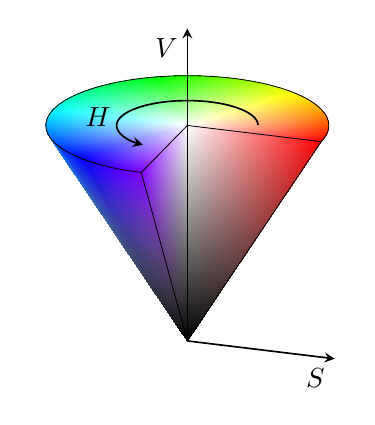
\begin{tikzpicture}[
	>=stealth,
]
		\def\arcbegin{0}
		\def\arcending{270}
	\begin{axis}[
		view={19}{30},
		axis lines=center,
		axis on top,
		domain=0:1,
		y domain=\arcbegin:\arcending,
		xmin=-1.5, xmax=1.5,
		ymin=-1.5, ymax=1.5,
		zmin=0.0, zmax=1.2,
		hide axis,
		samples=20,
		data cs=polar,
		mesh/color input=explicit mathparse,
		shader=interp,
	]
		% -----------------------------------------------------------------
		% also added the "color parts"
		% -----------------------------------------------------------------
		% cone:
		\addplot3 [
			surf,
			variable=\u,
			variable y=\v,
			point meta={symbolic={Hsb=v,u,u}},
		] (v,u,u);
		% top plane:
		\addplot3 [
			surf,
			samples=50,
			variable=\u,
			variable y=\v,
			point meta={symbolic={Hsb=v,u,1}},
		] (v,u,1);
		% slice plane
		\addplot3 [
			surf,
			variable=\u,
			y domain=0:1,
			variable y=\w,
			point meta={symbolic={Hsb=\arcbegin,u,z}},
		] (\arcbegin,u,{u+w*(1-u)});
		\addplot3 [
			surf,
			variable=\u,
			y domain=0:1,
			variable y=\w,
			point meta={symbolic={Hsb=\arcending,u,z}},
		] (\arcending,u,{u+w*(1-u)});
		% -----------------------------------------------------------------
		% border
		\addplot3 [
			line width=0.3pt,
		] coordinates {
			(0,0,0) (\arcbegin,1,1) (0,0,1)
			({(\arcending)},1,1) (0,0,0)
		};
		%%%%%%% border top
		\draw [line width = 0.3pt]
			(axis cs: {cos(\arcbegin)}, {sin(\arcbegin)},1)
%                arc (\arcbegin:\arcending:100)             % <-- old version
			arc (\arcbegin:\arcending:1)                % <-- new version
		;
		%%%%%%% arc
		\draw [->,line width = 0.6pt]
			(axis cs: {0.5*cos(\arcbegin+20)}, {0.5*sin(\arcbegin+20)},1)
%                arc ({\arcbegin+20}:{\arcending-20}:50)    % <-- old version
			arc ({\arcbegin+20}:{\arcending-20}:0.5)    % <-- new version
		;
		% x and z axis
		% \addplot3[
		% 	line width=0.6pt,
		% ] coordinates {
		% 	(\arcbegin,1.1,0)
		% 	(0,0,0)
		% 	(0,0,1.45)
		% };
        \draw [->,line width = 0.6pt] (0,0,0) -- (0,0,1.45);
        \draw [->,line width = 0.6pt] (0,0,0) -- (1.1,0,0);
		% annotations
		\node at (axis cs:1.1,0,0)      [anchor=north east] {$S$};
		\node at (axis cs:0,0,1.45)     [anchor=north east] {$V$};
		\node at (axis cs:-.5,0.0,1.0)  [anchor=east]       {$H$};

	\end{axis}
\end{tikzpicture}
    }\hspace{1cm}
    \subfigure[$RG$扇区]{
      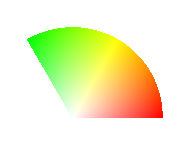
\begin{tikzpicture}[
        >=stealth,
      ]
      \pgfplotsset{width=5cm,height=5cm}
            \def\arcbegin{0}
            \def\arcending{120}
        \begin{axis}[
            view={0}{90},
            axis lines=center,
            axis on top,
            domain=0:1,
            y domain=\arcbegin:\arcending,
            xmin=-1.5, xmax=1.5,
            ymin=-1.5, ymax=1.5,
            zmin=0.0, zmax=1.2,
            hide axis,
            samples=60,
            data cs=polar,
            mesh/color input=explicit mathparse,
            shader=interp,
        ]
            \addplot3 [
                surf,
                samples=50,
                variable=\u,
                variable y=\v,
                point meta={symbolic={Hsb=v,u,1}},
            ] (v,u,1);
        \end{axis}
      \end{tikzpicture}
    }\hspace{1cm}
    \subfigure[$GB$扇区]{
      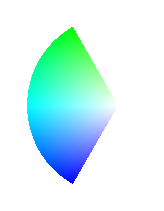
\begin{tikzpicture}[
        >=stealth,
      ]
      \pgfplotsset{width=5cm,height=5cm}
            \def\arcbegin{120}
            \def\arcending{240}
        \begin{axis}[
            view={0}{90},
            axis lines=center,
            axis on top,
            domain=0:1,
            y domain=\arcbegin:\arcending,
            xmin=-1.5, xmax=1.5,
            ymin=-1.5, ymax=1.5,
            zmin=0.0, zmax=1.2,
            hide axis,
            samples=60,
            data cs=polar,
            mesh/color input=explicit mathparse,
            shader=interp,
        ]
            \addplot3 [
                surf,
                samples=50,
                variable=\u,
                variable y=\v,
                point meta={symbolic={Hsb=v,u,1}},
            ] (v,u,1);
            \draw[white] (0,0) -- (0.2,0);
        \end{axis}
      \end{tikzpicture}
    }\hspace{1cm}
    \subfigure[$BR$扇区]{
      
\begin{tikzpicture}[
        >=stealth,
      ]
      \pgfplotsset{width=5cm,height=5cm}
            \def\arcbegin{240}
            \def\arcending{360}
        \begin{axis}[
            view={0}{90},
            axis lines=center,
            axis on top,
            domain=0:1,
            y domain=\arcbegin:\arcending,
            xmin=-1.5, xmax=1.5,
            ymin=-1.5, ymax=1.5,
            zmin=0.0, zmax=1.2,
            hide axis,
            samples=60,
            data cs=polar,
            mesh/color input=explicit mathparse,
            shader=interp,
        ]
            \addplot3 [
                surf,
                samples=50,
                variable=\u,
                variable y=\v,
                point meta={symbolic={Hsb=v,u,1}},
            ] (v,u,1);
        \end{axis}
      \end{tikzpicture}
    }
  \caption{HSI颜色模型与各扇区对应的色盘}
  \label{fig:4}
\end{figure}

综上所述,从HSI到RGB的变换为
$$
\left\{
  \begin{aligned}
    0^{\circ}&<H \leqslant 120^{\circ}\,,\\
    B&=I(1-S)\,,\\
    R&=I\left[1+\frac{S \cos H}{\cos \left(60^{\circ}-H\right)}\right]\,,\\
    G&=3I-R-B\,.
  \end{aligned}
\right.\quad
\left\{
  \begin{aligned}
    120^{\circ}&<H \leqslant 240^{\circ}\,,\\
    R&=I(1-S)\,,\\
    G&=I\left[1+\frac{S \cos\left(H-120^{\circ}\right)}{\cos \left(180^{\circ}-H\right)}\right]\,,\\
    B&=3I-R-G\,.
  \end{aligned}
\right.\quad
\left\{
  \begin{aligned}
    240^{\circ}&<H \leqslant 360^{\circ}\,,\\
    G&=I(1-S)\,,\\
    B&=I\left[1+\frac{S \cos\left(H-240^{\circ}\right)}{\cos \left(300^{\circ}-H\right)}\right]\,,\\
    R&=3I-G-B\,.
  \end{aligned}
\right.
$$
HSI颜色模型与各扇区对应的色盘如图~\ref{fig:4} 所示.

